% Supplementary Material --- BioSystems submission
% "Exhaustive circuit mapping of a single-cell foundation model reveals
%  massive redundancy, heavy-tailed hub architecture, and layer-dependent
%  differentiation control" (I. Kendiukhov)

\documentclass[10pt,letterpaper]{article}
\usepackage[margin=1in]{geometry}
\usepackage{amsmath,amssymb}
\usepackage{booktabs}
\usepackage{array}
\usepackage{graphicx}
\graphicspath{{figures/}}
\usepackage[labelfont=bf,labelsep=period]{caption}
\usepackage{url}
\usepackage[colorlinks=true,allcolors=blue]{hyperref}

\setlength{\parindent}{0pt}
\setlength{\parskip}{6pt}

% S-prefixed numbering for supplementary sections, figures, and tables
\renewcommand{\thesection}{S\arabic{section}}
\renewcommand{\thetable}{S\arabic{table}}
\renewcommand{\thefigure}{S\arabic{figure}}
\renewcommand{\figurename}{Fig}
\renewcommand{\tablename}{Table}

\title{\textbf{Supplementary Material}\\[4pt]
Supplementary methods, validation analyses, figures, and tables\\[8pt]
\large Exhaustive single-layer circuit mapping of a single-cell foundation model reveals
massive redundancy, heavy-tailed hub architecture, and layer-dependent steering directionality}
\author{Ihor Kendiukhov}
\date{}

\begin{document}
\maketitle


\section{Schematic of the four operations used in this paper}
\label{supp:schematic}

\begin{figure}[!ht]
\centering
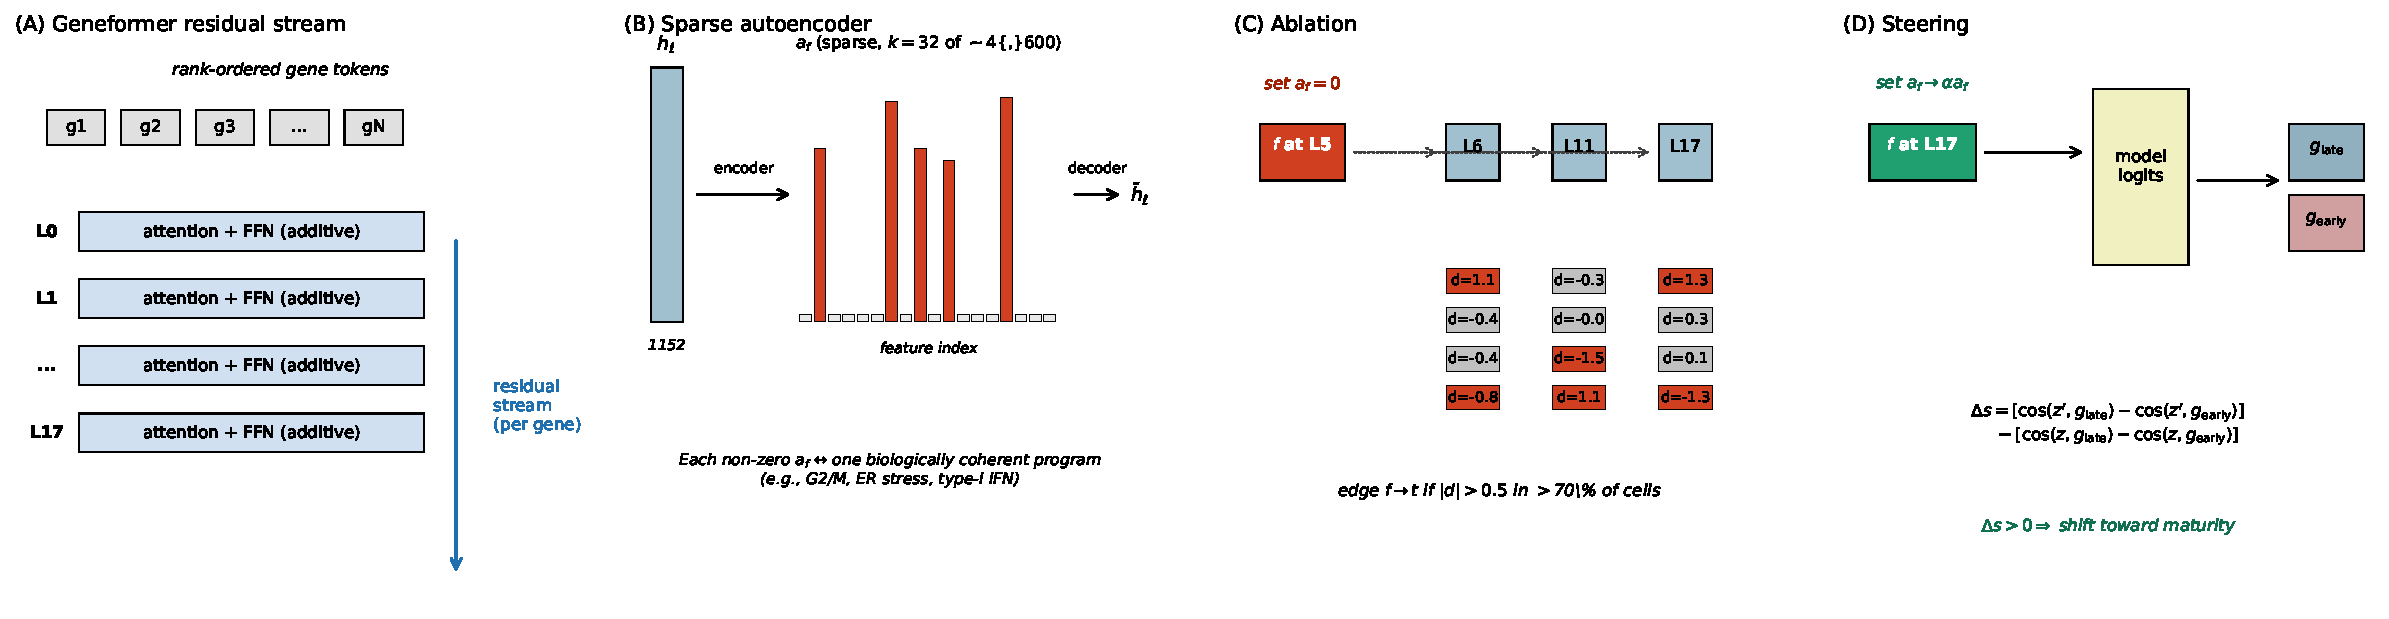
\includegraphics[width=0.85\textwidth]{S1_Fig.pdf}
\caption{\textbf{Schematic of the four operations.} (A)~Geneformer encodes a cell as rank-ordered gene tokens; the residual stream at each layer is a per-gene vector that the transformer additively rewrites. (B)~The SAE re-expresses each residual vector as a sparse combination of $\sim$4{,}600 ``feature'' directions, $\leq 32$ active per token. (C)~\emph{Ablation:} the coefficient for feature $f$ is set to zero; the modified residual is propagated and downstream activations compared against the clean pass (edge if $|d|>0.5$ in $>70\%$ of cells). (D)~\emph{Steering:} the coefficient is multiplied by $\alpha$; output logits shift, and we measure whether the shift is toward the late-pseudotime gene signature.}
\label{fig:schematic_supp}
\end{figure}


\section{Monosemanticity audit of layer-5 SAE features}
\label{supp:monosemanticity}

For 100 randomly sampled annotated L5 features:
\begin{enumerate}
\item \textbf{Top-gene/term Jaccard.} Mean Jaccard $\bar J = \mathbf{0.034}$, median $0.031$, versus a matched-size random-pair baseline of $\bar J_\mathrm{null} = 0.0023$---\textbf{14.6$\times$ enrichment}.
\item \textbf{Cross-context stability.} For 39 Hungarian-matched K562$\leftrightarrow$Tabula Sapiens SAE feature pairs (decoder cosine $>0.3$), mean top-50 gene-loading Jaccard is $\mathbf{0.13}$---feature identity is partially preserved across independent training contexts.
\end{enumerate}


\section{Source-layer sensitivity (L2, L8, L14)}
\label{supp:source_layer_sensitivity}

We re-ran the exhaustive-tracing protocol on 500 randomly sampled active features at three alternative source layers, each measured against three downstream layers $\{\ell+1, 11, 17\}$ (with $\{\ell+1, \ell+6, 17\}$ at L14):

\begin{center}
\begin{tabular}{lrrrrr}
\toprule
Source & \# feats & Mean edges & Median & Heavy-tail & Top-20 unann. \\
layer & traced & per feature & edges & ($\geq 1000$) & \\
\midrule
L2  & 500 & 377 & 301 & 3.8\% & 11/20 (55\%) \\
\textbf{L5} (main) & \textbf{4{,}065} & \textbf{343} & \textbf{284} & \textbf{1.8\%} & \textbf{8/20 (40\%)} \\
L8  & 500 & 358 & 290 & 3.4\% & 15/20 (75\%) \\
L14 & 500 & 390 & 288 & 3.6\% & 16/20 (80\%) \\
\bottomrule
\end{tabular}
\end{center}

Three qualitative findings replicate at every source layer:
\begin{enumerate}
\item \textbf{Heavy-tailed hub distribution.} Right-skewed at all four layers; heavy-tail fraction $1.8$--$3.8\%$. The maximum-hub edge count at L14 (2{,}842) exceeds the L5 maximum (2{,}138).
\item \textbf{Annotation and centrality.} The top-20 unannotated fraction is $40\%$ (L5), $55\%$ (L2), $75\%$ (L8), $80\%$ (L14). At L5 this is not a depletion relative to the $53.8\%$ background (Fisher's exact $p=0.66$; see the main-text enrichment tests); the depletion becomes significant only at L8 and L14. What is consistent across layers is that annotation status carries little information about a feature's degree, and the effect worsens with depth. At L14 the top thirteen hubs are all unannotated before the first annotated feature.
\item \textbf{Biological diversity of top hubs.} Chromatin/DDR/DNA-repair at L2 (F3540 \emph{Chromatin Remodeling}, F2256 \emph{DNA Damage Response}); RNA-processing/chromatin-remodeling at L8 (F3527 \emph{RNA Processing}, F4131 \emph{Chromatin Remodeling}); gene-expression/cell-cycle at L5; protein-modification/ribosome biogenesis at L14 (F50 \emph{Protein Modification}, F3994 \emph{Ribosome Biogenesis}). This shift from low-level (DNA) to high-level (translation, protein-modification) processes mirrors expected layer-wise hierarchical processing.
\end{enumerate}


\section{Downstream-layer completeness sweep}
\label{supp:downstream_completeness}

For the top 200 L5 hub features, we measured ablation effects on all 12 downstream layers (L6--L17). Mean significant edges per feature decline monotonically with depth:

\begin{center}
\begin{tabular}{rrrrrrrrrrrrr}
\toprule
DL & 6 & 7 & 8 & 9 & 10 & \textbf{11} & 12 & 13 & 14 & 15 & 16 & \textbf{17} \\
Edges/feature & \textbf{505} & 461 & 432 & 407 & 377 & \textbf{318} & 300 & 278 & 257 & 216 & 193 & \textbf{195} \\
\bottomrule
\end{tabular}
\end{center}

The decline is smooth and approximately log-linear; the main-trace sampling at $\{6, 11, 17\}$ corresponds to (top, middle, bottom) of this curve. L6$\to$L17 attenuation ratio is $2.6$, in line with the main-trace $2.7$.


\section{Cell-count power analysis}
\label{supp:cellcount_power}

For 48 features stratified by edge-count quartile, we ran the L5 protocol at varying $n$ with 3 independent random samples per $n$:

\begin{center}
\begin{tabular}{rrrr}
\toprule
$n$ & Mean edges/feature & Median & Test--retest $r$ \\
\midrule
5   & 472 & 346 & 0.98 \\
10  & 428 & 323 & 0.63 \\
\textbf{20}  & \textbf{347} & \textbf{271} & \textbf{0.91} \\
40  & 268 & 214 & 0.99 \\
80  & 212 & 174 & 0.99 \\
160 & 187 & 151 & 1.00 \\
\bottomrule
\end{tabular}
\end{center}

\emph{Calibration:} mean edges-per-feature at $n=20$ (347) matches the main exhaustive trace (mean 343, median 284) to within 1\%. \emph{Reliability:} test--retest $r$ at $n=20$ is $0.91$, comparable to $n=40$--$160$ ($r=0.99$--$1.00$). The dip at $n=10$ ($r=0.63$) and the artifactually high $r=0.98$ at $n=5$ bracket the regime in which $n=20$ is the cheapest stable choice. The monotonically decreasing mean edges with $n$ reflects the Cohen's $d$ threshold mechanism: higher $n$ tightens the SD and raises the bar to pass $|d|>0.5$.


\section{Cell-line generalization of L5 hubs}
\label{supp:celltype_generalization}

We re-ran the L5 tracing protocol restricted to the top-50 K562 hubs on 193 Tabula Sapiens immune cells:
\begin{itemize}
\item Spearman rank-correlation: $\rho=0.11$ ($p=0.45$). Pearson $r=0.11$ ($p=0.46$). Top-10 ranking agreement: 3/10.
\item Mean edges per hub: 1{,}344 in K562 vs.\ \textbf{25} in TS immune cells---a $\sim$50$\times$ drop.
\item \textbf{17/50 hubs ($34\%$) fire on zero TS cells}; median K562-hub active-cell count on TS immune cells is $5.5/193$. Only $8/50$ features ($16\%$) fire on $\geq 50$ TS cells.
\end{itemize}
\emph{Interpretation.} The collapse on TS data is dominated by an activation-frequency artifact: K562-trained SAE features are tuned to K562's transcriptomic distribution and frequently do not activate on immune-cell transcripts. A feature that does not fire cannot be ablated, so its downstream edge count is mechanically zero. The low rank-correlation does not imply that Geneformer's circuit architecture is cell-type-specific---only that \emph{the specific feature identities} of a K562-trained SAE do not transfer to TS immune cells. A definitive cell-type generalisation test requires training a separate SAE on TS immune-cell activations and tracing with it; we do this in Section~\ref{supp:ts_native}, which shows that the heavy-tailed, hub-dominated architecture and the annotation--centrality independence replicate with a natively trained TS SAE, while only the absolute edge density is cell-type-specific.


\section{Steering null baselines, ceiling, and precision floor}
\label{supp:steering_nulls}

This section reports the state-shift ($\Delta s$) null baselines for the \emph{original 14-feature panel}; the ``observed'' row is that panel's per-layer fraction-positive (hence L17 $=1.00$ across its 3 features). The expanded 80-feature panel, its ON/OFF directional control, dose--response and held-out readouts---which supersede the original panel's directionality summary---are in Section~\ref{supp:steering_full}, where the L17 fraction-positive on the expanded panel is $0.74$ on $\Delta s$ and $0.83$ on the held-out maturity probe.

Per-layer fraction-positive means at $\alpha=5$:

\begin{center}
\begin{tabular}{lrrrr}
\toprule
Distribution & L0 & L5 & L11 & L17 \\
\midrule
Switch features (observed) & 0.34 & 0.67 & 0.26 & \textbf{1.00} \\
Null A: random features (210) & 0.42 & 0.48 & 0.39 & 0.47 \\
Null B: random unit directions (14) & 0.43 & 0.36 & 0.29 & 0.48 \\
Null C: sign-shuffled (14) & 0.46 & 0.45 & 0.27 & 0.46 \\
Null 0: precision floor SD($\Delta s$) & \multicolumn{4}{c}{$0.0$ (bit-deterministic)} \\
\bottomrule
\end{tabular}
\end{center}

\begin{enumerate}
\item \textbf{Null A.} 210 non-switch features (32/54/67/57 per layer) under the same protocol. Per-layer fraction-positive is near chance ($0.39$--$0.48$), establishing that steered switch features exceed a random-feature baseline. (This null was computed on the original 14-feature panel; the expanded 80-feature panel, its ON/OFF control, dose--response and held-out readouts are in Section~\ref{supp:steering_full}, and supersede the ``$3/3$ at frac-pos $=1.0$'' summary for the directionality claim.)
\item \textbf{Null B.} Replace decoder direction with a unit-norm Gaussian. Fraction-positive $\in [0.29, 0.48]$; no L0$\to$L17 gradient.
\item \textbf{Null C.} Flip the sign of $(\alpha-1)$ for half the cells. Mean fraction-positive $\in [0.27, 0.46]$, per-feature SD $\leq 0.16$; metric unbiased.
\item \textbf{Null 0.} 50 repeated clean forward passes on 20 cells; SD$(\Delta s)=0$ exactly---MPS bit-deterministic in eval mode.
\end{enumerate}

The \emph{ceiling intervention} steers along $\hat g = \mathrm{proj}_{\mathrm{res}_\ell}(g_\text{late}-g_\text{early})$ scaled to the SAE-feature norm and to the maximum admissible norm; this bounds the maximum $\Delta s$ achievable under any single-direction perturbation:

\begin{center}
\begin{tabular}{lrr}
\toprule
Layer & SAE-norm $\Delta s$ & max-admissible $\Delta s$ \\
\midrule
L0  & 0.013 & 0.073 \\
L5  & 0.015 & 0.088 \\
L11 & 0.010 & 0.057 \\
L17 & 0.0005 & 0.0044 \\
\bottomrule
\end{tabular}
\end{center}

\begin{figure}[!ht]
\centering
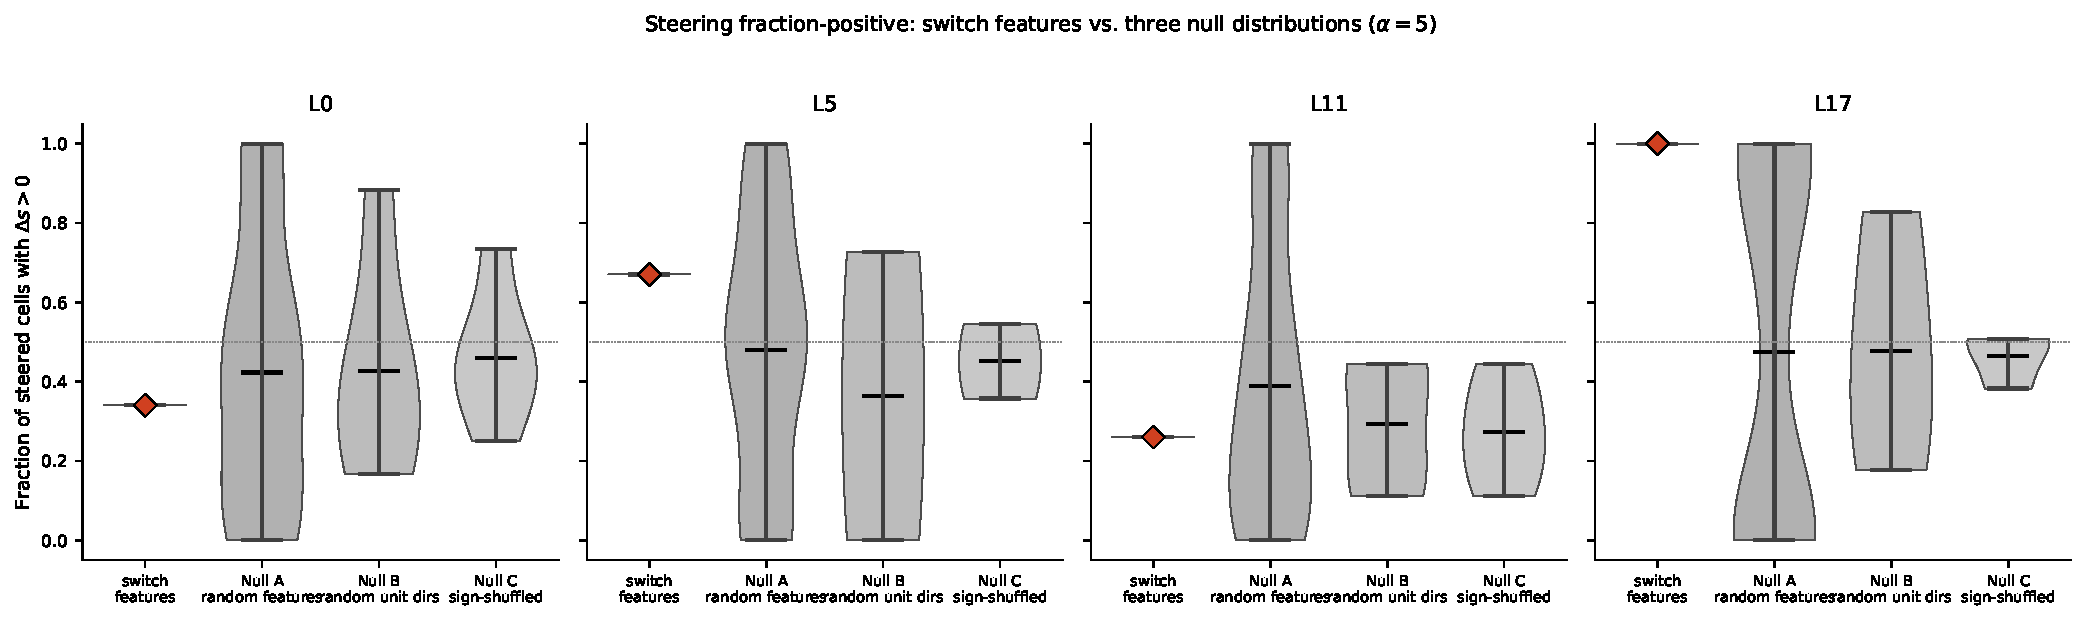
\includegraphics[width=0.85\textwidth]{S3_Fig.pdf}
\caption{\textbf{Steering effects against four nulls.} Per layer $\ell\in\{0, 5, 11, 17\}$, violin plots of fraction-positive across (i)~switch features (observed), (ii)~random features (Null~A), (iii)~random unit directions (Null~B), (iv)~sign-shuffled (Null~C). Ceiling shown as horizontal reference; precision-floor SD as annotation.}
\label{fig:steering_nulls_supp}
\end{figure}


\section{Annotation-pipeline validation}
\label{supp:annotation_validation}

\paragraph{(a) Null FPR.} 1{,}000 random gene sets of size 50 drawn from Geneformer's vocabulary were passed through the pipeline. \textbf{10/1{,}000 $=$ 1.0\%} received $q<0.05$ enrichment---well below the nominal $5\%$.

\paragraph{(b) Recall on canonical K562-active processes.}
We curated 29 GO/KEGG/Reactome terms covering canonical processes active in K562 cells (cell cycle, DNA replication/repair, RNA processing, translation, glycolysis, OxPhos, MAPK and PI3K-Akt signalling, apoptosis, autophagy, vesicle transport, etc.). Two complementary tests:
\begin{itemize}
\item \emph{Pipeline output coverage} (the practical metric): \textbf{27/29 $=$ 93\% coverage}; canonical processes are covered by multiple sub-terms (e.g., \emph{Mitotic Cell Cycle} by 17 labels, \emph{Apoptotic Process} by 20). Non-matches: \emph{Glycolysis} (no KEGG ``Glycolysis'' label assigned, although related metabolic features exist) and \emph{Protein Folding}.
\item \emph{Strict stress test} (Fisher's exact across all 4{,}065 features per canonical term, BH-corrected): \textbf{6/28 $=$ 21\%}; survivors are biologically high-prior processes (G2/M Transition, DNA Replication, OxPhos, MAPK signalling, Vesicle Transport, Reactome Cell Cycle). The gap reflects the conservatism of testing 4{,}065 features per term.
\end{itemize}

\paragraph{(c) Cross-context stability.}
To assess stability of the annotation pipeline under independent training, we compared the K562-trained L5 SAE against a Tabula Sapiens multi-tissue L5 SAE trained on a disjoint cell population---a stricter test than seed-to-seed stability, varying both seed and training distribution. Hungarian matching by decoder cosine ($>0.3$) yielded 39 matched pairs with mean top-50 gene-loading Jaccard $=0.13$, demonstrating partial preservation of feature identity across training contexts.


\section{Gene-level steering effects}
\label{supp:gene_effects}

\begin{figure}[!ht]
\centering
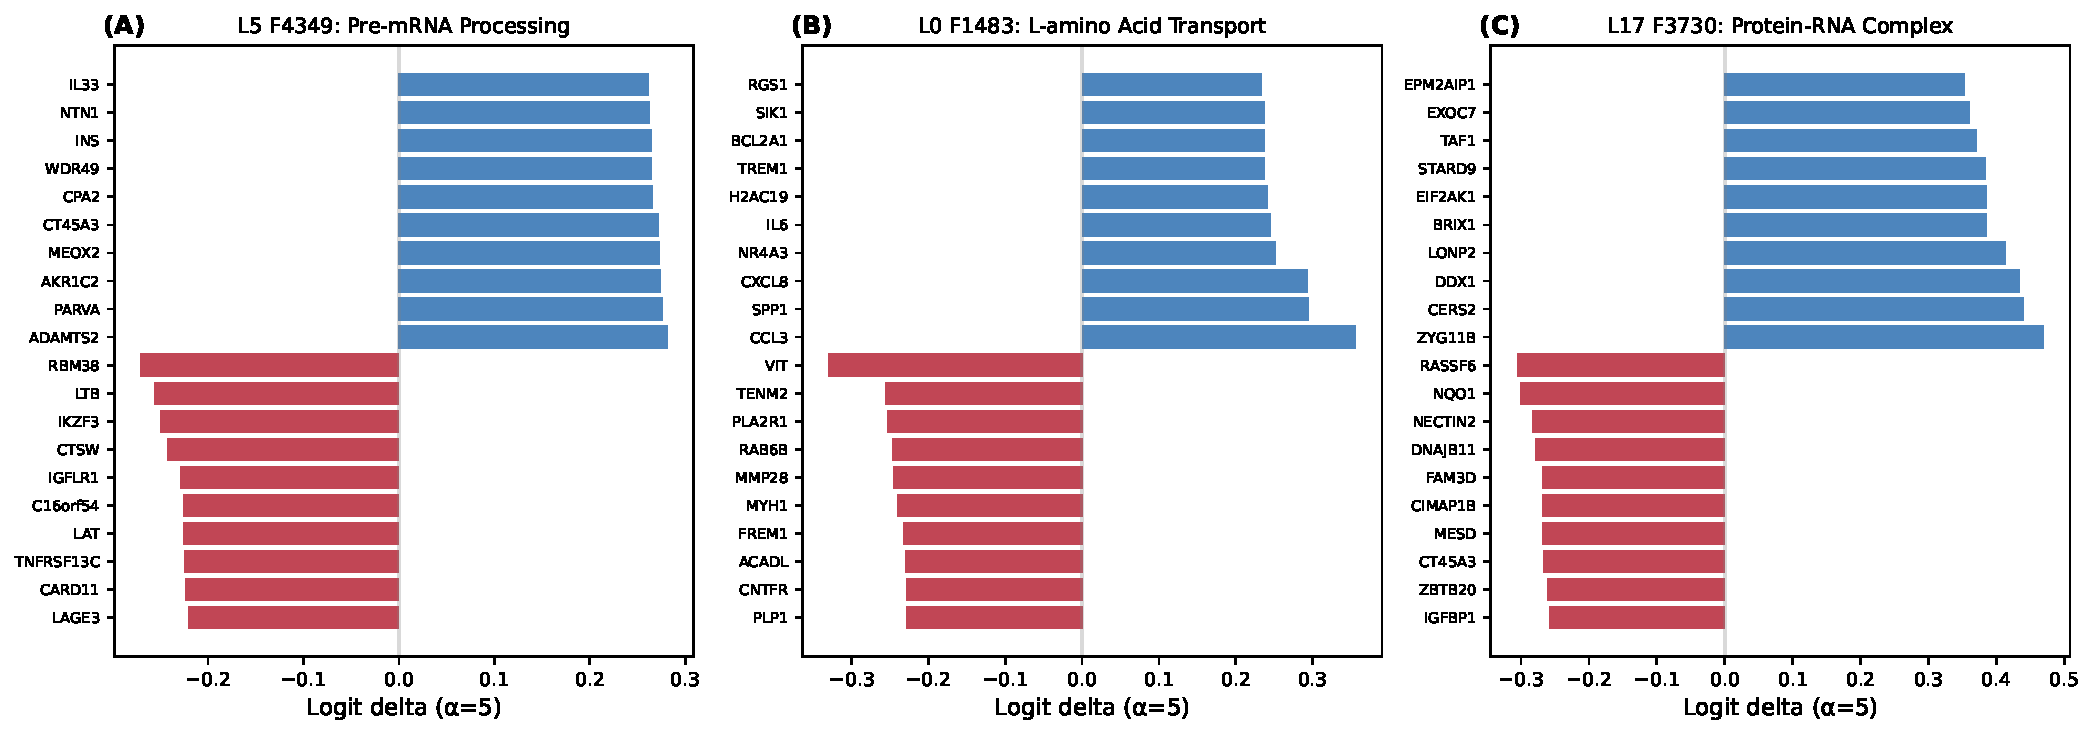
\includegraphics[width=0.85\textwidth]{S2_Fig.pdf}
\caption{\textbf{Gene-level steering effects at $\alpha=5$.} (A)~L5 F4349 (Pre-mRNA Processing): top 10 up- and downregulated genes. (B)~L0 F1483 (L-amino Acid Transport): top 10 genes. (C)~L17 F3730 (Protein-RNA Complex Assembly): top 10 genes.}
\label{fig:gene_effects}
\end{figure}


\section{The 14 previously published switch features}
\label{supp:switch_features}

The 14 features below are the panel reported in prior work. They are documented here for self-containment; the steering experiment in this paper uses the re-derived 80-feature panel (Section~\ref{supp:steering_full}), which contains all 14 as a subset. Switch $d$ values are as originally reported.

\begin{table}[!ht]
\centering
\caption{The 14 previously published switch features. Switch $d$: Cohen's $d$ between mean SAE activation in early- and late-pseudotime Tabula Sapiens immune cells, as originally reported; all 14 are higher in late.}
\label{tab:switch_features_supp}
\small
\begin{tabular}{rlrl}
\toprule
Layer & Feature & Switch $d$ & Annotation \\
\midrule
0 & F2061 & 1.33 & Chromatin Organization \\
0 & F25   & 1.13 & Mitotic Spindle Microtubule Attachment \\
0 & F3567 & 1.07 & \textit{unannotated} \\
0 & F1483 & 1.07 & L-amino Acid Transport \\
0 & F1295 & 1.01 & Neurodegeneration Pathways \\
5 & F4349 & 0.95 & Pre-mRNA Processing \\
5 & F2016 & 0.90 & \textit{unannotated} \\
11 & F854  & 1.15 & RNA Catabolic Process \\
11 & F4350 & 1.09 & \textit{unannotated} \\
11 & F2174 & 1.01 & \textit{unannotated} \\
11 & F3750 & 1.00 & \textit{unannotated} \\
17 & F3730 & 1.25 & Protein-RNA Complex Assembly \\
17 & F1607 & 1.09 & \textit{unannotated} \\
17 & F3567 & 1.09 & \textit{unannotated} \\
\bottomrule
\end{tabular}
\end{table}


\section{Summary schematic}
\label{supp:summary_schematic}

\begin{figure}[!ht]
\centering
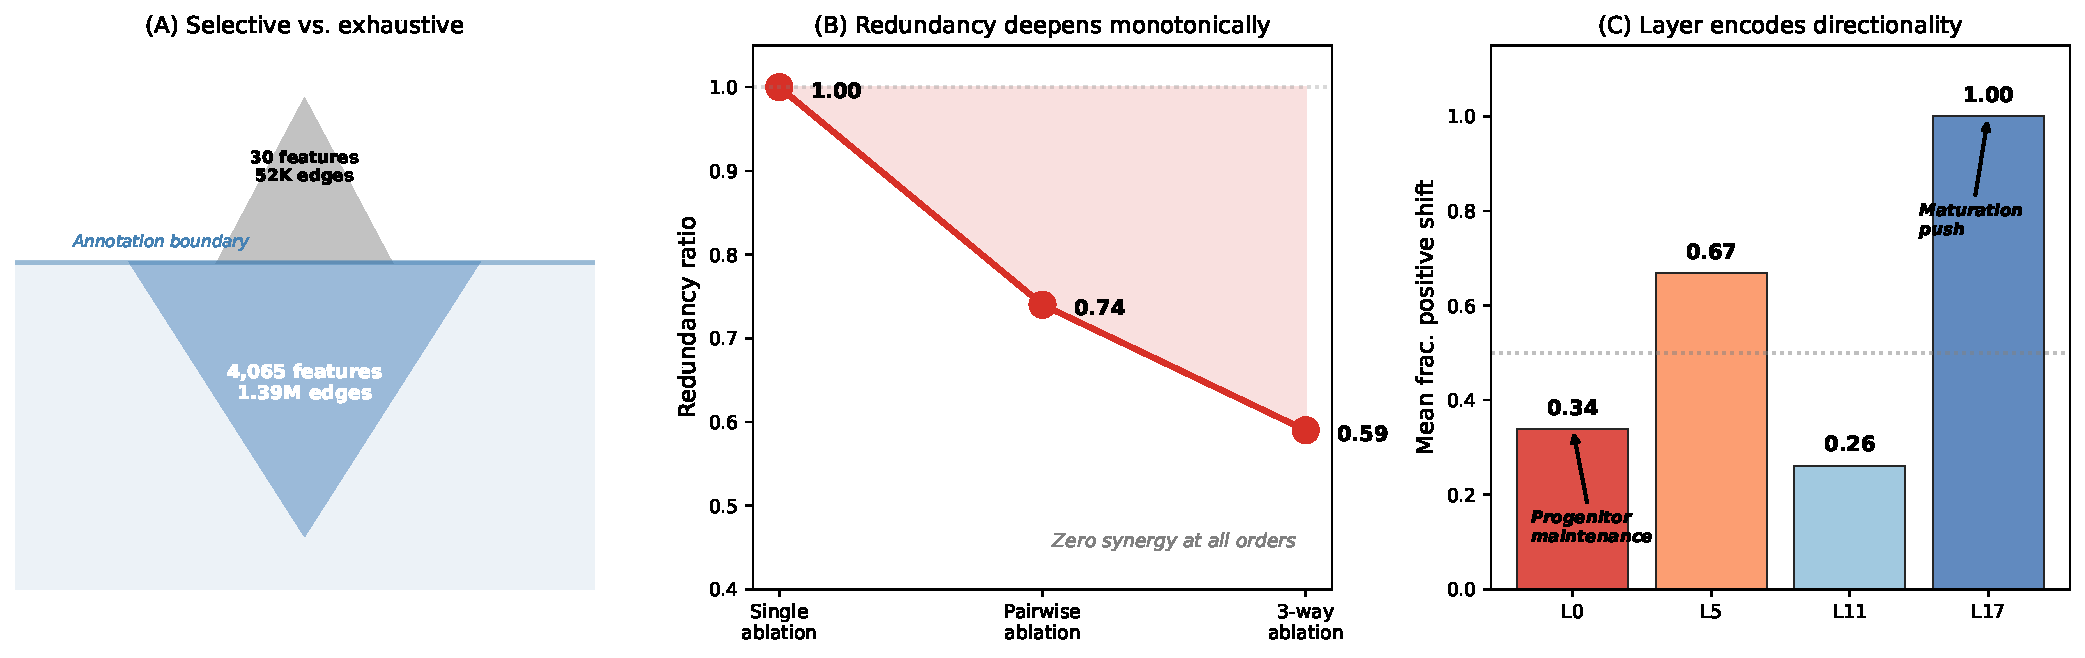
\includegraphics[width=0.85\textwidth]{S4_Fig.pdf}
\caption{\textbf{Summary of findings (schematic).} (A)~Selective tracing samples a small, annotation-selected part of the graph; exhaustive tracing exposes the rest, including high-degree features that current ontologies do not describe. (B)~The redundancy ratio decreases from single (1.0) to pairwise ($0.70$) to three-way ($0.53$) ablation; superadditive targets are rare ($<0.1\%$) and concentrated between pathways. (C)~Steering directionality is layer-dependent: at layer 17, ON-switch features shift a held-out maturity probe upward and OFF-switch features shift it downward, so the direction is carried by the feature rather than the layer. Panel values are illustrative; exact figures are in the main text.}
\label{fig:summary_schematic_supp}
\end{figure}



\section{Permutation null, FDR control, and threshold sensitivity for edge calling}
\label{supp:calibration}

\paragraph{Null.} Geneformer is deterministic, so a downstream feature on no path from the ablated feature has an exactly zero effect in every cell. Such targets are \emph{degenerate}: they cannot produce an edge and are excluded from the test family. For each live (source, target, downstream-layer) triple, the sign-flip null flips the sign of each cell's effect independently, $B=500$ times, and recomputes Cohen's $d$ and the consistency. It tests the hypothesis that the effect has no consistent direction across cells, conditioned on the observed magnitudes. The identity permutation is excluded from the null-edge count (it would reproduce the observed statistic and inflate the null by exactly $1/B$ of the observed count) and included, in the usual conservative form $p = (1+\#\{|d_\mathrm{perm}|\ge|d_\mathrm{obs}|\})/(1+B)$, in the permutation $p$-values.

\paragraph{Subset.} Permutation analysis was run on 600 features: the 200 highest-degree features, so that the hub table and top-20 ranking are exact, plus a degree-stratified random sample of 400. The calibrated total for all 4{,}065 features is obtained by applying each degree decile's surviving-edge ratio to the features whose degree falls in that decile.

\paragraph{Headline calibration.} On the 600-feature subset the criterion $|d|>0.5$, consistency $>0.7$ produces 327{,}609 edges against $11{,}915$ expected under the sign-flip null: an empirical false-discovery rate of $\mathbf{3.6\%}$. Of the 8{,}294{,}400 (source, target, downstream-layer) triples in the subset, 4{,}707{,}865 ($56.8\%$) are degenerate; of the 3{,}586{,}535 live tests, 1{,}090{,}165 ($30.4\%$) survive Benjamini--Hochberg at $q<0.05$. Requiring $q<0.05$ \emph{and} $|g|>0.5$ \emph{and} consistency $>0.7$ retains $261{,}564$ of the $303{,}507$ effect-size edges ($\mathbf{86.2\%}$). Applying each degree decile's survival ratio to all 4{,}065 active features gives a calibrated graph of $\approx 1{,}104{,}000$ edges ($79.2\%$ of $1{,}393{,}850$), mean $272$ edges per feature.

Under false-discovery control the hub set is essentially unchanged: 19 of the 20 highest-degree features are the same, the calibrated and uncalibrated degrees correlate at Spearman $\rho=0.99$ across the subset ($\rho=0.94$ within the top 200), the calibrated top-20 still contains 8 unannotated features, and the number of features with more than 1{,}000 edges falls from 72 ($1.8\%$) to 26 ($0.64\%$).

\paragraph{Threshold sweep.} Mean observed and expected-null edges per feature, the implied false-discovery rate, and the stability of the hub ranking against the default criterion. Both columns are computed on the same 600 features.

\begin{center}
\begin{tabular}{lrrrrr}
\toprule
Criterion & Edges/feat & Null/feat & FDR & Hub-rank $\rho$ & Top-20 kept \\
\midrule
\multicolumn{6}{l}{\emph{effect size, at consistency $>0.7$}}\\
$|d|>0.3$ & 1803 & 630.6 & 35.0\% & 0.954 & 17/20 \\
$\mathbf{|d|>0.5}$ & \textbf{546} & \textbf{19.9} & \textbf{3.6\%} & \textbf{1.000} & \textbf{20/20} \\
$|d|>0.8$ & 208 & 0.4 & 0.2\% & 0.964 & 18/20 \\
$|d|>1.0$ & 119 & 0.1 & 0.1\% & 0.911 & 15/20 \\
$|d|>1.5$ & 35 & 0.0 & 0.0\% & 0.647 & 9/20 \\
$|d|>2.0$ & 13 & 0.0 & 0.0\% & 0.508 & 5/20 \\
\midrule
\multicolumn{6}{l}{\emph{consistency, at $|d|>0.5$}}\\
$>0.6$ & 648 & 29.0 & 4.5\% & 0.993 & 19/20 \\
$\mathbf{>0.7}$ & \textbf{546} & \textbf{19.9} & \textbf{3.6\%} & \textbf{1.000} & \textbf{20/20} \\
$>0.8$ & 484 & 13.4 & 2.8\% & 0.994 & 19/20 \\
$>0.9$ & 425 & 8.2 & 1.9\% & 0.975 & 18/20 \\
$=1.0$ & 367 & 4.9 & 1.3\% & 0.939 & 16/20 \\
\bottomrule
\end{tabular}
\end{center}

The effect-size threshold does the work. At $|d|>0.3$ more than a third of the edges are noise; at $|d|>0.5$ the false-discovery rate falls by an order of magnitude at the cost of two thirds of the edges. The consistency threshold is a much weaker lever. Throughout the region with FDR below $5\%$ the hub ranking is stable (Spearman $\rho\geq0.91$; at least 15 of the top-20 preserved), so no structural conclusion in this paper depends on the exact threshold. Above $|d|>1.0$ the graph becomes too sparse for the ranking to be reliable.

\paragraph{Numerical precision of the archived deltas.} The per-cell effect vectors are archived as float16. Recomputing degrees from them rather than from the float64 originals changes the total edge count by $9.8\times10^{-5}$ of edges (mean $-0.02$ edges per feature; maximum $2$ for any single feature). All statistics in this section are computed from the archived arrays.

\begin{figure}[!ht]
\centering
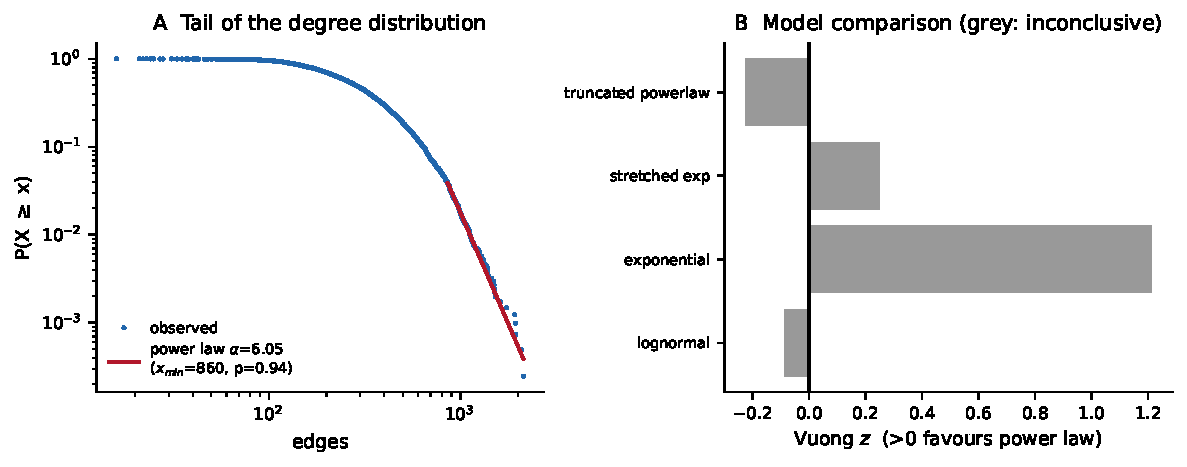
\includegraphics[width=0.9\textwidth]{S7_Fig.pdf}
\caption{\textbf{The degree distribution is heavy-tailed but not scale-free.} (A)~Complementary cumulative distribution of feature degree (log--log) with the maximum-likelihood power-law fit above $x_\mathrm{min}=860$ ($\alpha=6.05$, 157 tail points). (B)~Vuong likelihood-ratio tests of the power law against four alternatives; grey bars ($|z|<1.3$, $p>0.2$) indicate the data cannot discriminate.}
\label{fig:tailfit}
\end{figure}


\paragraph{Norm-matched specificity control.} The sign-flip null asks whether an edge could have arisen without a consistently directed effect. It does not ask whether the edge is specific to the ablated feature. For 200 features stratified by degree decile, we replaced the ablation displacement $\Delta h = \mathrm{dec}(h_{f=0})-\mathrm{dec}(h)$ with a Gaussian random direction rescaled to the same per-position $L_2$ norm and repeated the measurement.

For 200 features spanning all ten degree deciles we substituted a Gaussian random direction of matched per-position $L_2$ norm for the ablation displacement. Real ablations produced a mean of $355.6$ edges per feature (median $283$) against $22.7$ (median $20$) for the norm-matched direction---a $15.7\times$ ratio, with $93.6\%$ of the total edge mass attributable to feature identity (Wilcoxon signed-rank $p=2.3\times10^{-34}$). The norm-matched edge count is itself weakly degree-dependent (Spearman $\rho=0.42$ against the observed degree), which is expected if high-degree features tend to occupy higher-variance residual-stream directions; it does not account for the bulk of the graph.


\section{Steering: full panel, dose--response, and readout concordance}
\label{supp:steering_full}

\paragraph{Panel construction.} Switch features are re-derived from the 481-cell Tabula Sapiens SAE activation matrices. Cells are split at the terciles of diffusion pseudotime (160 early, 160 late). For every feature with activation frequency $\geq 0.05$ we compute Cohen's $d$ between late and early terciles with pooled standard deviation. The panel is the top 12 ON-switch ($d\geq0.5$) and top 8 OFF-switch ($d\leq-0.5$) features at each of layers 0, 5, 11 and 17. All 14 features of the previously published panel lie inside this set (they occupy ON-switch ranks 1--6 at their respective layers).

\paragraph{Cell counts.} A feature can be steered only in cells where it fires. Median cells per feature among the 160 early-pseudotime cells: 27 (L0 ON), 110 (L0 OFF), 16 (L5 ON), 72 (L5 OFF), 23 (L11 ON), 57 (L11 OFF), 66 (L17 ON), 77 (L17 OFF). Five features fire in fewer than 10 cells (2 at L5 ON, 3 at L11 ON) and are excluded from all reported statistics; 75 of 80 remain. ON-switch features are systematically rarer than OFF-switch features, which is a direct consequence of selecting for higher activation in the late tercile and steering in the early one.

\paragraph{Dose--response.} Twenty-nine features (four per layer per switch direction, minus exclusions) were measured at $\alpha\in\{1.5,2,3,5,8\}$. Because most features push \emph{away} from maturity, the signed effect decreases with $\alpha$ for them; the meaningful question is whether the magnitude grows and the sign is preserved. It is: the number of features whose $|$effect$|$ increases monotonically with $\alpha$ (Spearman $\rho>0.8$) is 27/29 ($\Delta s$), 27/29 (marker score), 25/29 ($\Delta P(\mathrm{terminal})$), 25/29 (predicted pseudotime); the sign is constant across the entire dose range for 22, 29, 24 and 27 of 29 features respectively. Median $\rho(\alpha, |{\rm effect}|) = 1.00$ for all four readouts.

\paragraph{ON versus OFF, per layer (Mann--Whitney $U$, two-sided, $\alpha=5$).}

\begin{center}
\begin{tabular}{lrrrr}
\toprule
Layer & $\Delta s$ & Marker score & $\Delta P(\mathrm{terminal})$ & $\Delta$ pseudotime \\
\midrule
L0  & 0.47 & 0.73 & 0.47 & 0.12 \\
L5  & 0.83 & 0.27 & 0.76 & 0.57 \\
L11 & 0.89 & 0.37 & 0.48 & \textbf{0.015} \\
L17 & \textbf{0.039} & 0.27 & \textbf{0.0055} & 0.24 \\
\bottomrule
\end{tabular}
\end{center}

Only at layer 17 do ON- and OFF-switch features separate on both the pseudotime-derived metric and an independent probe, and there they separate in the direction the switch label predicts.

\paragraph{Layer gradient among ON-switch features ($\alpha=5$).} Spearman correlation between layer index and mean effect: $+0.36$ ($p=0.017$) for $\Delta P(\mathrm{terminal})$; $+0.23$ ($p=0.15$) for $\Delta s$; $+0.06$ ($p=0.71$) for predicted pseudotime; $-0.18$ ($p=0.25$) for the marker score.

\paragraph{Readout concordance.} Across the 75 features, $\Delta s$ correlates \emph{negatively} with the literature marker score (Spearman $\rho=-0.43$, $p=6.5\times10^{-5}$; sign agreement 36\%) and only weakly with the maturity probe ($\rho=+0.17$, $p=0.14$) and the pseudotime probe ($\rho=+0.01$, $p=0.93$). Within layer 17 alone, $\Delta s$ agrees with the maturity probe ($\rho=+0.67$, $p=0.0013$). By contrast, $\Delta s$ recomputed from a bone-marrow-only signature reproduces the pooled value at $\rho=0.92$, and from a blood-and-spleen-only signature at $\rho=1.00$. The metric is stable with respect to which cells define the signature and unstable with respect to what the signature is taken to mean.

\paragraph{Marker panels.} Progenitor: CD34, KIT, FLT3, MPO, GATA2, SPINK2, PROM1, CRHBP, AVP, HLF, MECOM, AZU1, ELANE, CTSG, TCF7, LEF1, SELL, CCR7. Terminal maturation: LYZ, S100A8, S100A9, S100A12, FCN1, CSF3R, FCGR3B, ITGAM, CD14, CST3, GNLY, NKG7, PRF1, GZMB, MS4A1, CD79A, JCHAIN, MZB1. All 36 map to Geneformer tokens. The marker score is the mean change in output logit over the terminal panel minus the mean change over the progenitor panel.

\paragraph{Held-out probes.} The maturity probe is a logistic regression on Geneformer's mean-pooled final-layer embedding, trained on 670 labelled Tabula Sapiens hematopoietic cells drawn from a 1{,}500-cell pool disjoint from the 481 steered cells (57 immature, 630 terminal by cell-type ontology); five-fold cross-validated AUC $=0.838\pm0.032$. The pseudotime probe is ridge regression from clean embeddings to diffusion pseudotime, fit on the 321 cells outside the early tercile; five-fold cross-validated $R^2=0.33$. Neither probe sees the SAE, the switch labels, or the steering.


\section{Higher-order ablation: extended triplet panel}
\label{supp:triplets_full}

Twelve triplets were run at 100 cells per condition with one feature at each of layers 0, 5 and 11, measured at layer 17. Same-pathway triplets take the highest-frequency annotated feature of one pathway at each layer; cross-pathway triplets take three different pathways; random triplets draw features frequency-matched to the others and are redrawn if any two share an annotated pathway. Features are ablated sequentially along the forward pass, each re-encoded on the already-perturbed residual stream, exactly as in the pairwise and published three-way protocols.

Confidence intervals on the redundancy ratio are percentile bootstrap intervals over \emph{targets} (1{,}000 resamples), which is the unit the median is taken over. Resampling cells instead would perturb every effect-size estimate --- duplicated cells shrink the within-cell standard deviation and inflate $|d|$ --- and produces intervals that do not cover the point estimate. Superadditive rates are given with Wilson intervals.

\begin{center}
\small
\begin{tabular}{llllrl}
\toprule
Class & Pathways & Features & $R_{ABC}$ & 95\% CI & Superadd. \\
\midrule
same pathway & vesicle & L0\,F2905, L5\,F2630, L11\,F1724 & 0.560 & [0.544, 0.579] & 0/594 \\
same pathway & translation & L0\,F4148, L5\,F3797, L11\,F1305 & 0.529 & [0.503, 0.547] & 0/642 \\
same pathway & rna & L0\,F4201, L5\,F2520, L11\,F4576 & 0.482 & [0.454, 0.499] & 1/726 \\
same pathway & metabolism & L0\,F2834, L5\,F4473, L11\,F1835 & 0.571 & [0.551, 0.586] & 0/641 \\
cross pathway & ddr $\times$ mitosis $\times$ mitosis & L0\,F561, L5\,F1762, L11\,F1023 & 0.527 & [0.513, 0.538] & 4/920 \\
cross pathway & vesicle $\times$ metabolism $\times$ translation & L0\,F2905, L5\,F4473, L11\,F1305 & 0.530 & [0.508, 0.544] & 1/837 \\
cross pathway & translation $\times$ ddr $\times$ rna & L0\,F4148, L5\,F671, L11\,F4576 & 0.526 & [0.512, 0.540] & 0/525 \\
cross pathway & metabolism $\times$ translation $\times$ ddr & L0\,F2834, L5\,F3797, L11\,F3904 & 0.561 & [0.536, 0.589] & 0/401 \\
random & random & L0\,F3134, L5\,F1686, L11\,F2316 & 0.532 & [0.504, 0.562] & 0/307 \\
random & random & L0\,F750, L5\,F2270, L11\,F1119 & 0.528 & [0.494, 0.548] & 1/605 \\
random & random & L0\,F1066, L5\,F4204, L11\,F3380 & 0.491 & [0.465, 0.543] & 0/173 \\
random & random & L0\,F1918, L5\,F2674, L11\,F1835 & 0.611 & [0.593, 0.632] & 0/554 \\
\bottomrule
\end{tabular}
\end{center}

Pooled by class: same-pathway $R_{ABC}=0.544$, 1/2{,}603 superadditive ($0.038\%$); cross-pathway $R_{ABC}=0.529$, 5/2{,}683 ($0.186\%$); random $R_{ABC}=0.530$, 1/1{,}639 ($0.061\%$). Median pairwise ratio across all 12 triplets is $0.699$; median three-way ratio is $0.530$; median marginal effect of the third feature, $|d_{ABC}|-|d_{AB}|$, is $0.115$ (range $0.001$--$0.431$).

Fisher's exact tests on superadditive counts: cross-pathway versus same-pathway OR $=4.86$, $p=0.22$; cross-pathway versus random OR $=3.06$, $p=0.42$; same-pathway versus random OR $=0.63$, $p=1.0$. The cross-pathway enrichment points the way the previously published single cross-pathway triplet did, but four triplets per class cannot resolve a difference between rates of $0.04\%$ and $0.19\%$.

Two features of the table matter more than the pooled numbers. Random triplets, whose features share no annotated pathway, are as subadditive as same-pathway triplets: redundancy is not a property of shared biological function in this model. And no triplet of any class has a redundancy ratio near 1: even three unrelated directions in the residual stream carry substantially overlapping information about their downstream targets.


\section{Model-internal importance of hub features}
\label{supp:hub_importance}

We ablated one feature at a time and measured Geneformer's masked-gene-prediction loss on 50 held-out K562 control cells (cells 100--149 of the control block, disjoint from the 20 used for tracing), with 15\% of gene tokens masked. Mask positions were drawn once and reused across all arms so that every feature is evaluated on identical inputs. Three arms of 50 features each: the 50 highest-degree layer-5 features (hubs); 50 randomly drawn non-hub features; and 50 non-hub features matched one-to-one to the hubs on log activation frequency.

\begin{center}
\begin{tabular}{lrrr}
\toprule
Arm & $\Delta$ cross-entropy (mean) & (median) & $\Delta$ top-1 accuracy (mean) \\
\midrule
Hub              & $+0.0005$ & $-0.0002$ & $-0.00014$ \\
Frequency-matched & $-0.0038$ & $+0.0006$ & $+0.00011$ \\
Random           & $-0.0015$ & $\phantom{+}0.0000$ & $+0.00007$ \\
\bottomrule
\end{tabular}
\end{center}

Baseline masked-LM cross-entropy is $5.42$ and top-1 recovery accuracy is $0.154$. All effects are within $10^{-3}$ of zero, and the median change is not even consistently positive: removing a single SAE feature from a residual stream of $\sim$4{,}600 features essentially never degrades masked prediction, which is the expected behaviour of a deeply redundant model.

The relevant test is not the mean but the correlation between degree and damage across features. It is negative: Spearman $\rho=-0.40$ ($p=3\times10^{-7}$) between log-degree and change in cross-entropy, and $\rho=-0.48$ ($p=3\times10^{-10}$) after partialling out log activation frequency. Hub features are not more damaging to ablate than random features (Mann--Whitney $p=0.998$ testing the fragility direction); the only arm that separates from random is the frequency-matched one, and it separates in the protective direction. Higher-degree features are more robust to ablation, not more fragile.

\begin{figure}[!ht]
\centering
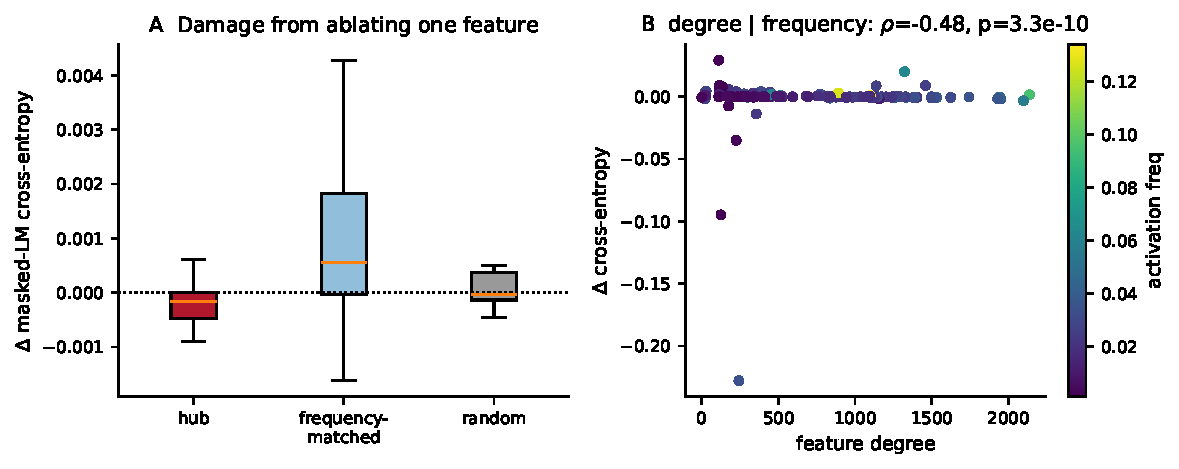
\includegraphics[width=0.85\textwidth]{S5_Fig.pdf}
\caption{\textbf{Hub features are not fragile.} (A)~Change in masked-LM cross-entropy from ablating one feature, for the hub, frequency-matched and random arms. (B)~Per-feature damage against degree, coloured by activation frequency; degree and damage are negatively associated once frequency is controlled.}
\label{fig:hubimp}
\end{figure}


\section{Tracing with a natively trained Tabula Sapiens SAE}
\label{supp:ts_native}

We repeated the tracing protocol on Tabula Sapiens immune cells using an SAE trained natively on Tabula Sapiens activations (available at layers 0, 5, 11 and 17), tracing 400 active layer-5 features on 20 immune cells at downstream layers 11 and 17. The K562 trace is restricted to the same two downstream layers for comparison.

\begin{center}
\begin{tabular}{lrr}
\toprule
& TS-native SAE & K562 SAE \\
\midrule
Features traced & 400 & 4{,}065 \\
Mean edges/feature & 9.6 & 172 \\
Median edges/feature & 0 & 144 \\
Max edges & 172 & 1{,}183 \\
Gini of degree & 0.90 & 0.34 \\
Skewness of degree & 3.1 & 2.2 \\
Fraction $>5\times$ median & 13.8\% & 0.4\% \\
Annotation rate & 51.5\% & 53.8\% \\
Top-20 unannotated & 70\% & 40\% \\
Spearman(freq, degree) & 0.16 & 0.79 \\
Spearman(degree, annotated) & $-0.14$ & $+0.16$ \\
\bottomrule
\end{tabular}
\end{center}

Two things replicate and two do not. The heavy-tailed, hub-dominated \emph{shape} is present and if anything stronger with a native SAE (higher Gini, higher skewness, larger heavy-tail fraction), and annotation does not predict centrality (a slightly negative correlation, matching the deeper K562 layers). The absolute edge \emph{density} collapses (mean 9.6 versus 172; the median native feature has no significant edges), and the frequency--degree coupling weakens. Both reflect the immune population being far more transcriptionally homogeneous than proliferating K562 cells: fewer SAE features fire, and those that fire do so on a narrower range of cells, so few ablations clear the $|d|>0.5$ threshold. The circuit architecture is a property of the model under an SAE decomposition; its scale is set by the cell population. The earlier report of near-zero hub-ranking agreement between K562 and immune cells is therefore an activation-frequency artefact, not evidence that Geneformer's circuit organisation is cell-type-specific.

\begin{figure}[!ht]
\centering
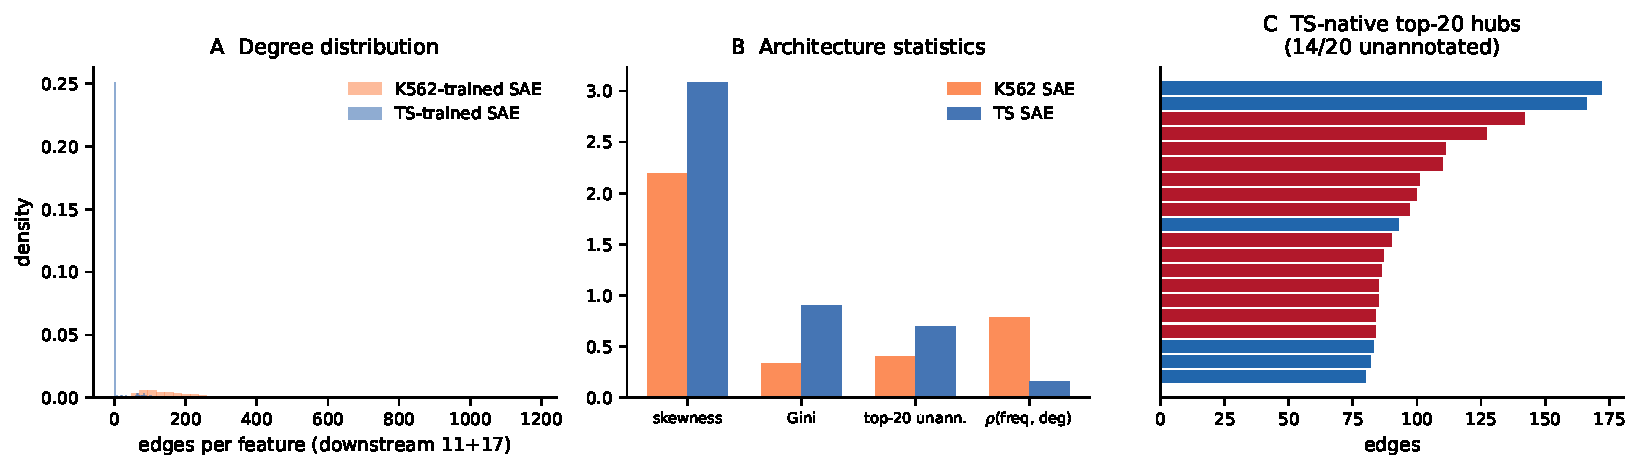
\includegraphics[width=0.95\textwidth]{S6_Fig.pdf}
\caption{\textbf{Hub architecture survives a change of SAE training context.} (A)~Degree distributions of the K562-trained and Tabula Sapiens-trained SAEs on the same downstream layers. (B)~Architecture statistics: the native SAE is more concentrated (higher Gini and skewness). (C)~Top-20 native hubs; red bars are unannotated.}
\label{fig:tsnative}
\end{figure}


\section{CRISPRi grounding of feature degree}
\label{supp:crispri}

For each of 2{,}023 K562 CRISPRi perturbations with at least 20 cells (Replogle et al., 2022), we computed the Euclidean distance between the perturbation's pseudobulk profile and the non-targeting control profile in log-normalised expression space. Because that distance grows as the number of cells shrinks, it was standardised against a null built by resampling non-targeting cells into pseudo-perturbations of matched size, giving a shift $z$-score (median $z=31.9$, interquartile range $19.9$--$48.6$). Each layer-5 feature was assigned the mean $z$ of those of its top-50 loading genes present in the screen; 2{,}384 features had at least five such genes.

\begin{center}
\begin{tabular}{lrr}
\toprule
Association with CRISPRi shift $z$ & Spearman $\rho$ & $p$ \\
\midrule
Feature degree & $+0.021$ & 0.30 \\
Feature degree (gene-label permutation null, 500 perms) & --- & 0.44 \\
Feature degree, partialling out activation frequency and mean expression & $-0.013$ & 0.54 \\
Frequency-residualised degree & $-0.024$ & 0.24 \\
Mean expression of the feature's top genes & $+0.087$ & $2\times10^{-5}$ \\
\bottomrule
\end{tabular}
\end{center}

Hub features (top 1.8\% by degree, $n=43$) have mean shift $z=37.0$ against $35.5$ for the remaining 2{,}341 (Mann--Whitney $p=0.19$). The only quantity that predicts how strongly a knockdown perturbs the K562 transcriptome is how highly expressed the gene is, which is a property of the gene and not of the model.


\end{document}
